%==================================================================================================
%   LUKES THESIS TEMPLATE 1.2
%   -------------------------
%   This template is based upon the offcial IMM PhD Thesis template, it is enhanced with a number
%   of new features and a number of errors have fixed. This template is intended to be complied to
%   PDF using PDFLATEX and is tested using the MiKTeX 2.9 LaTeX distribution.
%   It is based on the official DTU-IMM Thesis template by Finn Kuno Christensen in 2009.
%   Small bugfixes by Kasper Laursen in 2012 and 2013.
%   Small updates by Finn Kuno Christensen/Henning Christiansen in 2015.
%   -------------------------
%   Last Updated: 2015-01-08
%==================================================================================================
%
%==================================================================================================
% DOCUMENT SETUP
%==================================================================================================
\documentclass[10pt,twoside]{book}                  %Official DTU-IMM Thesis document setup
%
%Set to 'print' for printed version, use 'net' for online version
\def\thesisversion{print}
%
%==================================================================================================
% PACKAGES
%==================================================================================================
\usepackage{LukeThesis}                             %Import Thesis base style
%input{PhDMacros}                                   %Thesis specific macros
%
%==================================================================================================
% THESIS PROPERTIES (Modifiy these fields with your details)
%==================================================================================================
\def\thesisauthor{Morten Chabert Eskesen}                     %Author
\def\thesistitle{Fault-tolerant architecture design for flow-based biochips}               %Title
\def\thesishandin{26-June}                       %Submission date (Day-Month}
\def\thesisdegree{MSc}                              %Degree ('B.Eng', 'B.Sc.', 'M.Sc.' or 'PhD')
\def\thesisyear{2015}                               %Submission year
\def\thesisnumber{????}                             %DTU-IMM Serial number (do not include year)
\def\thesisISSN{0000-0000}                          %ISSN number
\def\thesiskeywords{Keywords are, comma separated}  %PDF keywords
\derivethesisprops                                  %Derive dependent properties
%
%==================================================================================================
% SECTION NUMBERING SETUP
%==================================================================================================
\setcounter{tocdepth}{2}                            %2 adds sections up to subsections
\setcounter{secnumdepth}{3}                         %Subsubsections get a number when this is 3
%
%==================================================================================================
% THESIS STRUCTURE  (Modifiy to include more chapters etc)
%==================================================================================================
\begin{document}
%------------------------
%Pre-frontmatter material
%------------------------
\prefrontmatter
%--------------------
%Frontmatter material
%--------------------
\frontmatter
\pagenumbering{roman}                               %Set frontmatter numbering style
\chapter{Summary (English)}

Microfluidic biochips revolutionise biology by placing laboratory functionality on a very small chip. In this thesis, the focus is on flow-based biochips. Flow-based microfluidic biochips are used for the manipulation of continuous fluid through fabricated microchannels, using external pressure sources or integrated mechanical micro-pumps. In these biochips, the basic building block is a microvalve, which can be fabricated at very high densities, e.g., 1 million valves per cm$^2$ \cite{wajid}. By combining these valves, more complex units such as mixers, switches and multiplexers can be built. Flow-based biochips are manufactured using multilayer soft lithography.

A potential roadblock in the deployment of microfluidic biochips is the lack of test techniques to screen defective devices before they are used for biochemical analysis. Defective chips lead to repetition of experiments. This is undesirable due to high reagent cost and limited availability of samples. Flow-based biochips are also affected by faults, and the defects can escape the after-fabrication inspection and can thereby affect the operation. Recent work has addressed fault-modeling and the automated testing of flow-based biochips.

Based on these fault models and testing techniques, the objective of this thesis is to propose approaches for the fault-tolerant design of flow-based biochips, such that the biochips can tolerate several permanent faults, given a cost budget and a biochip area. During the physical design of the biochip layout, redundancy can be introduced for on-chip components such as valves, channels and microfluidic units in order to improve fault-tolerance, thereby increasing thus the yield.

The thesis proposes a fault model as part of the biochip architecture model and introduces a component library with fault-tolerant components. Using these models, two algorithmic approaches to solving the problem of fault-tolerant architecture synthesis are proposed. The fault-tolerant architecture synthesis considers the application model, fault-tolerant routing and the physical constraints of the biochip such that the minimum amount of redundancy is added to achieve fault-tolerance. The proposed approaches have been evaluated using real-life case studies and synthetic benchmarks.                                   %English summary of Thesis
\markboth{}{}                                       %Set headings (left)(right)
\chapter{Summary (Danish)}
\begin{otherlanguage}{danish}

Mikrofluidiske biochips revolutionerer biologi ved at lægge laboratorie funktionalitet på en meget lille chip. Denne afhandling fokuserer på flow-baserede biochips. Flow-baserede mikrofluidiske biochips er baseret på behandling af kontinuerlig væske gennem fabrikeret mikrokanaler ved at bruge eksterne trykkilder eller integreret mikro-pumper. I disse biochips er byggestenen en mikrovalve som kan blive fabrikeret ved høj tæthed, fx. 1 million valves per cm$^2$. Ved at kombinere disse valves kan mere komplekse enheder fremstilles - herunder mixere, switches, multipleksere. Flow-baserede biochips er fremstillet ved brug af multilags blød litografi.

En potentiel forhindring i implementeringen af mikrofluidiske biochips er manglen på testteknikker til at screene defekte enheder før de bruges til biokemisk analyse. Defekte chips fører til gentagelse af eksperimenter. Dette er uhensigtsmæssigt på grund af høje reagens omkostninger og begrænset tilgængelighed af prøver. Flow-baserede biochips er også påvirket af fejl, og disse defekter kan undslippe efter-fabrikation inspektion og dermed påvirke operationen. Fejlmodellering og automatiske test af flow-baserede biochips er blevet adresseret fornyligt i en teknisk rapport.

Baseret på disse fejlmodeller og fejlfindingsteknikker er målet for denne afhandling at foreslå tilgange til det fejltolerante design af flow-baserede biochips således at biochippen kan tolerere flere permanente fejl givet et budget og et biochip område. Under det fysiske design af biochippens layout kan redundans introduceres for komponenterne på chippen såsom valves, kanaler og microfluidiske enheder, og derved øge udbyttet af biochips.

Denne afhandling foreslår en fejlmodel som en del af biochip arkitekturmodellen og introducerer et komponentbibliotek med fejltolerante komponenter. Ved brug af disse modeller er to algoritmiske tilgange foreslået til at løse problemet med fremstilling af fejltolerante arkitekturer. Fremstillingen af fejltolerante arkitektur tager applikationsmodellen og fejltolerant rutebestemmelse på biochippen med i overvejelserne samt de fysiske begrænsinger således at den minimale mængde af redundans er tilføjet for at opnå fejltolerance. De foreslåede tilgange er blevet evalueret ved brug af real-life case studies og syntetiske benchmarks.

\end{otherlanguage}                                   %Danish summary of Thesis
\markboth{}{}                                       %Set headings (left)(right)
\chapter{Preface}

This thesis was prepared at DTU Compute in fulfilment of the requirements for acquiring an M.Sc. in Engineering.

The thesis deals with ...

The thesis consists of ...
%==================================================================================================
% SIGNATURE AREA
%==================================================================================================
\vspace{20mm}
\begin{center}
    \hspace{20mm} Lyngby, \thesishandin-\thesisyear
    \vspace{5mm}
    \newline
  %Update signature image file in line below
    
\includegraphics[scale=0.5]{figures/SignatureDummy}
\end{center}
\begin{flushright}
    \thesisauthor
\end{flushright}
% % % EOF % % %                                     %Preface
\markboth{}{}                                       %Set headings (left)(right)
\chapter{Acknowledgements}

Firstly, I would like to thank my supervisor Paul Pop for his close involvement and excellent guidance throughout my work which have been extremely helpful. His capability to always be available for questions and discussion contributed a great deal in the completion of this thesis.

Secondly, I want to thank my colleague Andreas Hallberg Kjeldsen, who has been an invaluable partner throughout my studies for five years and contributed with small algorithmic ideas for this thesis.

Lastly, I want to extend my gratitude to my family who have supported and encouraged me. I dedicate this thesis to my brother, Julian, who has been and will always be my inspiration in life.                            %Acknowledgements
\markboth{}{}                                       %Set headings (left)(right)
%------------------
% Table of contents
%------------------
\newpage\mbox{}\newpage
\chaptermark{Contents}
\pdfbookmark{\contentsname}{toc}
\renewcommand{\sectionmark}[1]{\markright{#1}}
\sectionmark{Contents}
\addtolength{\parskip}{-\baselineskip}
\tableofcontents
\addtolength{\parskip}{\baselineskip}
\renewcommand{\sectionmark}[1]{\markright{\thesection\ #1}}
%-------------
% Main content
%-------------
\mainmatter
\chapter{Introduction}
Microfluidics is the science of handling and manipulating very small volumes of fluids. It is a multidisciplinary field that involves engineering, physics, chemistry, biochemistry, nanotechnology, and biotechnology. Microfluidic biochips combine different biochemical analysis functionalities, e.g. mixers, filter, detectors, on-chip. It miniaturises the macroscopic chemical and biological processes to a sub-millimetre scale \cite{microfluidic-largescale}.  
\\
There are several types of microfluidic biochip platforms. Based on the fluid manipulation on the chip, biochips can broadly be divided into two categories \cite{wajid}.
\begin{itemize}
\item Droplet-based biochips
\item Flow-based biochips
\end{itemize}
In this thesis the focus is on flow-based biochips. The following sections will explain the flow-based technology and its application areas.

\section{Flow-based Biochips}
Flow-based biochips are fabricated using multilayer soft lithography. \autoref{fig:flow-based-biochip} shows a flow-based biochip. Polydimethylsiloxane, \emph{PDMS}, is used as the fabrication substrate \cite{integration-microfluidics}. PDMS is used as it is a cheap and rubber-like elastomer with good biocompatibility and optical transparency.
\begin{figure}[H]
\centering
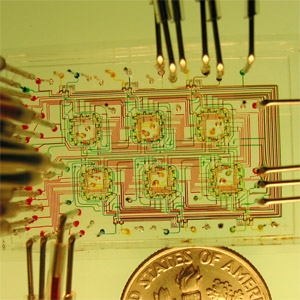
\includegraphics[scale=0.65]{figures/flow-based-biochip.jpg}
\caption[Flow-based biochip]{Flow-based biochip \cite{stanford-group}.}
\label{fig:flow-based-biochip}
\end{figure}

Flow-based biochips can have multiple physical layers, but the layers are logically divided into two types: \emph{flow layer} and \emph{control layer}. The flow layer is depicted in blue and the control layer in red as shown in \autoref{fig:flow-based-concept}a. The liquid is in the flow layer and it is manipulated using the control layer \cite{integration-microfluidics}.

\begin{figure}[H]
\centering
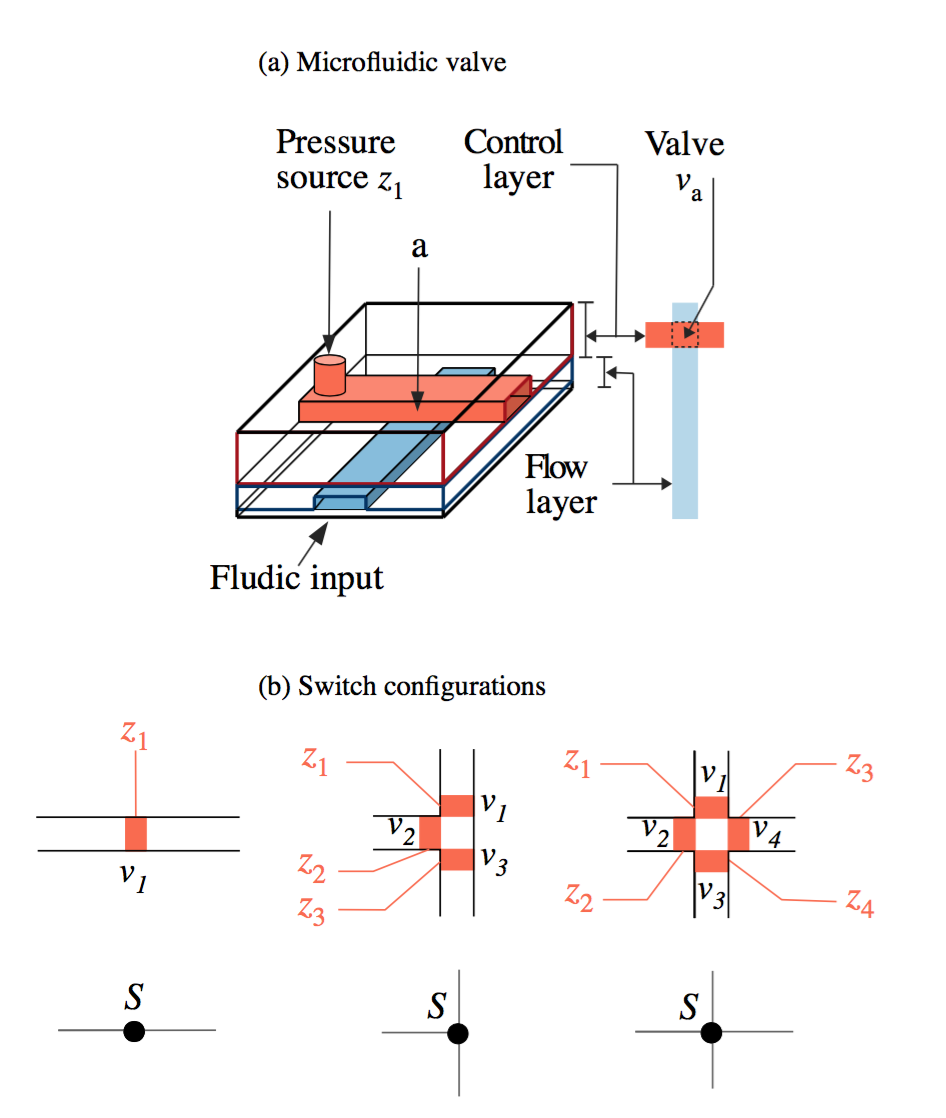
\includegraphics[scale=0.425]{figures/flow-based-concept.png}
\caption[Flow-based valve and switch]{Flow-based valve and switch \cite{wajid}.}
\label{fig:flow-based-concept}
\end{figure}

A valve (shown in \autoref{fig:flow-based-concept}a) is the basic building block of such a biochip. The control layer is connected to an external air pressure source through the punch hole $z_1$. This is referred to as a control pin. The flow layer is connected to a fluid reservoir through a pump which generates the fluid flow. When the external air pressure in the control layer is not active, the fluid is permitted to flow freely, i.e. the valve is open. When the pressure source is activated, the high pressure causes the elastic control layer to pinch the underlying flow layer (point $a$ in \autoref{fig:flow-based-concept}a) blocking the fluid flow, i.e. the valve is closed. These valves are used to manipulate fluids in the flow layer as the valves either restrict or permit the fluid flow. More complex units such as switches, mixer, micropumps, etc., can be formed by combining these valves. An example of valves combining to form a component is that of a switch. Three different switch configurations are depicted in \autoref{fig:flow-based-concept}b. As shown here a switch can consist of one or more valves. Multiple valve switches are present at channel junctions and are used to control the path of the fluids entering the switch from different sides. The fluid flow can be generated by either using off-chip or on-chip pumps. The control layer is not necessarily above the flow layer as shown in \autoref{fig:flow-based-concept}a. It can also be below the flow layer by creating a "push-up" valve, and having the control layer above the flow layer is done by creating a "push-down" valve. The connections to external ports (fluidic ports for the flow layer and pressure sources for the control layer) are made by punching holes in the chip and placing external tubings into the punch holes \cite{integration-microfluidics}. All input ports are connected to the off-chip pumps.

\subsection{Application Areas}
Since the introduction of this technology, several biochips have been designed which target a variety of biochemical applications \cite{life-sciences-microfluidics}. A few are listed below:

\begin{itemize}
\item \emph{Microreaction Technology}: These chips allow the production of fine chemicals. The superior mixing and reaction control properties of microfluidic systems are used to perform chemical reaction or syntheses at much better yields and better selectivity than in conventional systems. Chemical reactions can take place much faster by reducing the diffusion length \cite{life-sciences-microfluidics}.

\item \emph{Cell Biology}: As the typical dimensions of cells are 5-20 $\mu m$, it is an ideal size for the size range of typical microfluidic structures. The applications within cell biology range from the observation of the physical and biological behaviour of single cells in different culturing media, chemotaxis experiments to observations of growth patterns, the guidance of growth. This can potentially be of great importance in drug research \cite{life-sciences-microfluidics}.

\item \emph{Diagnosis Testing}: Certain chips allow the diagnosis of diseases. Known examples are chips testing for Human Immunodeficiency Virus (\emph{HIV}) and syphilis \cite{wajid}. The chip designed for this purpose is cheap, easy to use, requires only micro-litres of the blood sample and it simultaneously tests for HIV and syphilis producing the result within 20 minutes \cite{wajid}.

\end{itemize}


One of the biggest beneficiaries of microfluidic devices and systems is the diagnostic market, especially molecular diagnostics. Microfluidics and miniaturisation technologies have a crucial enabling role for new product development in this field due to the required integration density, portability and speed for such applications can only be realised in miniaturised solutions. Additionally, many of the diagnostic procedures require the integration of methods of molecular biology like DeoxyriboNucleic Acid (DNA) extraction or Polymerase Chain Reaction (PCR) which can only be performed in their microfluidics-based protocols outside a specialised laboratory \cite{life-sciences-microfluidics}.

\section{Motivation}
A potential roadblock in the deployment of microfluidic biochips is the lack of test techniques to screen defective devices before they are used for biochemical analysis. Defective chips lead to repetition of experiments. This is undesirable due to high reagent cost and limited availability of samples. %Flow-based biochips are also affected by faults, and the defects can escape the after-fabrication inspection and can thereby affect the operation.
Recent work has addressed the fault-modeling and the automated testing of flow-based biochips \cite{fault-modeling}.

Based on these fault models and testing techniques, the objective of this thesis is to propose approaches for the fault-tolerant design of flow-based biochips, such that the biochips can tolerate several permanent faults, given a cost budget and a biochip area. During the physical design of the biochip layout, redundancy can be introduced for on-chip components such as valves, channels and microfluidic units to improve fault-tolerance, thereby increasing thus the yield.

This thesis explores techniques and algorithms for designing fault-tolerant flow-based biochips. The purpose is to design and implement a tool to assist the designer in designing a fault-tolerant biochip. Implementing such a tool requires a biochip architecture model, biochemical application model, heuristics for introducing fault-tolerance and a way to evaluate the fault-tolerance of the biochip.
%The remaining chapters elaborate these topics, formulate the exact problem, and evaluate the tool on a set of benchmarks.

\subsection{Related Work}
In \cite{wajid} there are proposed system models for flow-based biochips which are used in this thesis. The proposed models used in this thesis are the biochip architecture model and the biochemical application model. Additionally, \cite{wajid} also contributes towards application mapping, architectural synthesis and control synthesis for flow-based biochips.

The physical placement of components is done by the designer of the flow-based biochip, which is a time-consuming and error-prone phase. In \cite{michael}, an automated tool for the physical placement of components is proposed which assists the designer in choosing the best placement.

Fault-tolerant design of microfluidic biochips has been done in \cite{mirela}. However, the thesis in \cite{mirela} introduces fault-tolerant design for droplet-based biochips. The thesis proposes algorithms to generate application-specific biochip architectures that are able to tolerate a certain number of permanent faults. The aim of the thesis was to increase the yield of fabricated biochips.


\section{Thesis Overview}
This thesis is organised in eight chapters. A brief summary of the chapters are provided here.

\begin{description}
\item[Chapter 2] presents the different types of faults in flow-based biochips and an automated testing strategy to determine the faults and locations thereof in a flow-based biochip.

\item[Chapter 3] describes the system models used in this thesis and proposes a fault-model for flow-based biochips. Furthermore it outlines the problem of application mapping.

\item[Chapter 4] focuses on the fault-tolerant architecture synthesis problem for flow-based biochips. It proposes two algorithmic solutions to obtain a fault-tolerant architecture.

\item[Chapter 5] proposes an evaluation method for architectures in order to determine if a given architecture is fault-tolerant.

\item[Chapter 6] describes the implementation of the tool developed in this thesis.

\item[Chapter 7] experimentally evaluates the proposed algorithmic approaches on a number of benchmarks. The evaluation is done in terms of solution quality and performance of the algorithms.

\item[Chapter 8] presents the conclusions of this thesis and the options for future work.

\end{description}
\chapter{Faults in Flow-Based Biochips}

\section{Possible Faults and Causes}

\section{Defects}

\section{Fault Modeling}

\section{Testing Strategy}

\section{Summary}
\chapter{System Models}

\section{Biochip Architecture Model}

\subsection{Component Model}

\subsection{Architecture Model}

\subsection{Fault Model}

\section{Biochemical Application Model}

\section{Application Mapping}

\section{Benchmarks}

\section{Summary}
\chapter{Architectural Synthesis}

\section{Problem Formulation}

\section{Alternative Architecture Generation}

\section{Simulated Annealing Architecture Synthesis}

\subsection{Concept}

\subsection{Design Transformations}

\subsection{Implementation}

\section{GRASP Architecture Synthesis}

\subsection{Concept}

\subsection{Implementation}

\section{Summary}
\chapter{Architecture Evaluation}
\label{chap:arch-eval}
This chapter focuses on architecture evaluation. The chapter will define how an alternative architecture generated by SA and GRASP is evaluated. The objective function consists of three parts: graph connectivity, scheduling of the application onto the architecture and the cost of the architecture. These three parts will be explained in detail in this chapter.

\section{Objective Function}
Before evaluating an architecture the set of fault scenarios, $\mathcal{FS}$, must be randomly generated from the fault model $\mathcal{Z} = (\mathcal{VF}, \mathcal{CF}, v, c)$. The number of fault scenarios is given by the designer. The generated fault scenarios are iterated and each iteration applies a fault scenario to the architecture, i.e. the faults in the fault scenario are injected into the architecture (see \autoref{fig:faultscenario}). In each iteration the connectivity of the architecture, $ft$, and the finish time, $\delta$, of the application on the architecture are determined. The architecture evaluation is then the sum of three variables.
$$Objective(\mathcal{A}) = \left(\displaystyle\sum_{f \in \mathcal{FS}}^{\mathcal{FS}}{\neg ft}\right) \times W_{ft} + \left(\displaystyle\sum_{f \in \mathcal{FS}}^{\mathcal{FS}}{max(0, \delta - d_{\mathcal{G}})}\right) \times W_{s} + Cost_{\mathcal{A}}$$

$\left(\displaystyle\sum_{f \in \mathcal{FS}}^{\mathcal{FS}}{\neg ft}\right)$ is the number of fault scenarios that causes the architecture to not be connected. Connectivity is denoted by $ft$ where $ft$ will be 1 if the architecture is connected and 0 if it is not connected. The number is then multiplied with $W_{ft}$ which denotes a penalty value for the connectivity. Consequently this variable will become smaller the more fault scenarios that pass the connectivity test. The penalty value $W_{ft}$ is specified as 10000.

$\left(\displaystyle\sum_{f \in \mathcal{FS}}^{\mathcal{FS}}{max(0, \delta - d_{\mathcal{G}})}\right)$ denotes the scheduling of the application on the architecture affected by the different fault scenarios. In each fault scenario the maximum of either 0 or the application finish time minus the application deadline is added to the sum. Thereby the sum grows larger as the application is not schedulable on the architecture or if it completes after the deadline. The sum is then multiplied with $W_s$ which denotes a penalty value for the schedule. Therefore the variable will grow larger as the application is not able to complete within its deadline or no schedule has been found. The penalty value $W_s$ is defined as 5000.

$Cost_{\mathcal{A}}$ denotes the physical constraints. This variable is the sum of the total number of valves and the total number of channels in the architecture.

\begin{figure}
\centering
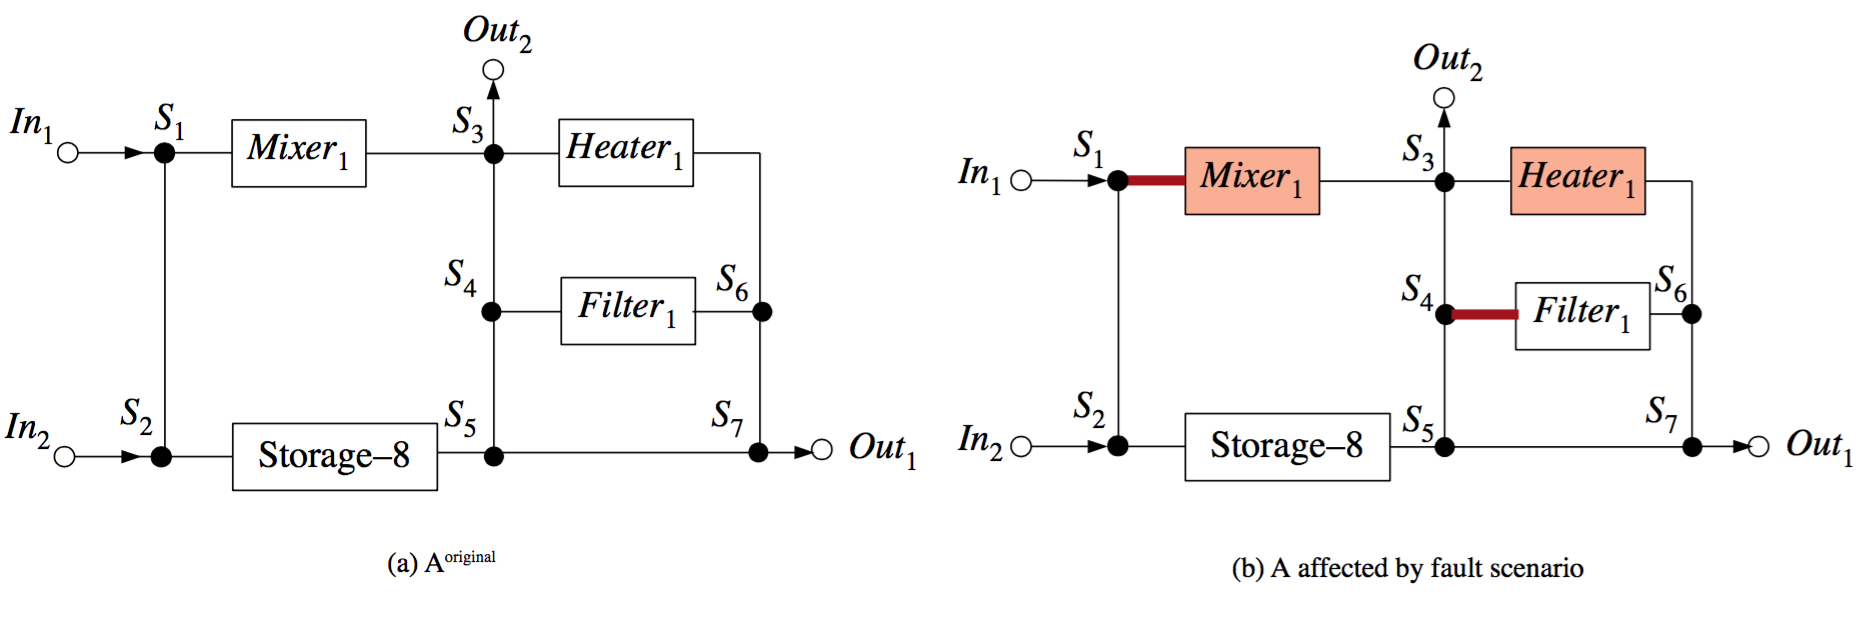
\includegraphics[width=\textwidth]{figures/faultscenario.png}
\caption[Architecture affected by fault scenario]{Architecture affected by fault scenario}
\label{fig:faultscenario}
\end{figure}

Let us consider \autoref{fig:faultscenario}a as the architecture to be evaluated, $\mathcal{A}^{original}$. Consider the fault scenario, where the channel $S_1 \rightarrow Mixer_1$ is blocked and the channel of $Heater_1$ suffers from a block defect. Additionally valves $v_6$ (a valve in the pump) of $Mixer_1$, $v_1$ (channel towards $S_3$) and $v_3$ (channel towards $S_5$) of $S_4$ are stuck open. The effects of this fault scenario is shown in \autoref{fig:faultscenario}b, where channels marked with a thick red line represent unusable channels and components marked with red are unable to perform their operation. Therefore we are unable to perform mixing, heating and route to $Filter_1$. This injection of the faults in a fault scenario is done for all generated fault scenarios, and the connectivity and scheduling are determined for each fault scenario.

The following sections will describe how the fault scenarios are generated, how the connectivity of the architecture is determined and how scheduling the application onto the architecture is done.

\section{Generation of Fault Scenarios}
\label{sec:fs-gen}
The fault scenarios, $\mathcal{FS}$, are randomly generated from the fault model $\mathcal{Z} = (\mathcal{VF}, \mathcal{CF}, v, c)$. A fault scenario $f \in \mathcal{FS}$ is a set of faults containing a set of valve faults from the set of valve faults, $\mathcal{VF}$, in the fault model and a set of channel faults from the set of channel faults, $\mathcal{CF}$, in the fault model. The fault scenarios are generated such that they are unique, i.e. $f \in \mathcal{FS}$ will occur once and only once.

The random generation of fault scenarios is divided into two phases.\\
\begin{description}
\item[First phase] The first phase consists of generating all the possible combinations of subsets of both the set of valve faults, $\mathcal{VF}$, and the set of channel faults, $\mathcal{CF}$. Recall that $v$ is the maximum number of valve faults happening in the architecture at any point and likewise $c$ is the maximum number of channel faults. Therefore all permutations of the set of valve faults needs to be generated where cardinality of the subsets are $0 \leq k \leq v$. Likewise for the set of channel faults where the cardinality of the subsets are $0 \leq j \leq c$.

\item[Second phase] The second phase picks a random subset from all the possible combinations of subsets of valve faults. Similarly it picks a random subset from the subsets of channel faults. Combining these two subsets constitutes a fault scenario, $f \in \mathcal{FS}$. This continues until the specified number of fault scenarios to generate are generated.

\end{description}

Normally we would have to use all the fault scenarios when doing the tests for connectivity and scheduling. However, as these are too numerous we have decided to use a subset. By virtue of this we are not guaranteed to create a fault-tolerant architecture which is fault-tolerant to all scenarios. However, our argument is that by using a subset, we can synthesise an architecture that can tolerate most of the fault scenarios. This argument has been investigated in \autoref{chap:exp-eval}. However, it is not a problem if an architecture is not fault-tolerant. As mentioned in \autoref{sec:prob-for} this tool is part of a methodology. If after testing we determine that a fault, which is not tolerated, is present, we will discard the chip.

The implementation of the generation of fault scenarios is shown in \autoref{alg:fault-gen-algo}. $NoFS$ is the number of fault scenarios to be generated.

\begin{figure}[H]
\centering
\begin{algorithmic}[1]
\Function{GenerateFaultScenarios}{$\mathcal{Z}, NoFS$}
	\State $vsubsets \gets \Call{PossibleCombinations}{\mathcal{VF}, v}$\Comment{Phase 1}
	\State $csubsets \gets \Call{PossibleCombinations}{\mathcal{CF}, c}$
	\State $i \gets 0$
	\State $\mathcal{FS} \gets \emptyset$
      \While{$i < NoFS$}\Comment{Phase 2}
        \State $v \gets \Call{RandomSet}{vsubsets}$
        \State $c \gets \Call{RandomSet}{csubsets}$
        \State $f \gets v \cup c$
	\If{$f \notin \mathcal{FS}$}\Comment{If the fault scenario does not exist add it to $\mathcal{FS}$}
		\State $\mathcal{FS}.\Call{add}{f}$
		\State $i \gets i + 1$
	\EndIf
      \EndWhile
      \State \textbf{return} $\mathcal{FS}$
    \EndFunction

\Function{PossibleCombinations}{$set, k$}
	\State $j \gets 1$
	\State $subsets \gets \emptyset$
	\While{$j \leq k$}
		\State $r \gets \Call{permutations}{set, j)}$
		\State $subsets.\Call{add}{r}$
	\EndWhile
	\State $subsets.\Call{add}{\emptyset}$\Comment{Remember that the empty set (no faults) is possible}
	\State \textbf{return} $subsets$
\EndFunction
\end{algorithmic}
\caption[Implementation of random generation of fault scenarios]{Implementation of random generation of fault scenarios}
\label{alg:fault-gen-algo}
\end{figure}

\section{Connectivity}
\begin{figure}
\centering
\begin{algorithmic}[1]
\Function{IsConnected}{$\mathcal{A}$}
	\State $start \gets \Call{ChooseRandomInput}{\mathcal{A}}$
	\State $visited \gets \emptyset$\Comment{Keep track of the visited components}
	\State $Q.\Call{enqueue}{start}$\Comment{$Q$ is a FIFO queue}
	\State $visited.\Call{add}{start}$
      \While{$Q$ is not empty}
        \State $v \gets Q.\Call{dequeue}{\null}$
	\ForAll{connection from v to w in $\mathcal{A}$.OutConnections(v)}
		\If{connection not faulty and $w \notin visited$}
		\State $visited.\Call{add}{w}$
		\State $Q.\Call{enqueue}{w}$
		\EndIf
	\EndFor
      \EndWhile
	%\State $inputs \gets \mathcal{A}.inputs$ \textbackslash ${}$ $start$\Comment{A set containing all components excluding inputs}
	\If{($\mathcal{N}$ $\backslash$ $\mathcal{A}.inputs$) $\in visited$}\Comment{If all vertices $N \in \mathcal{N}$ excluding inputs are in the $visited$ set. The architecture is connected}
		\State \textbf{return} true
	\Else
		\State \textbf{return} false
	\EndIf
    \EndFunction
\end{algorithmic}
\caption[Implementation of graph connectivity algorithm]{Implementation of graph connectivity algorithm}
\label{alg:connectivity}
\end{figure}
Due to permanent faults, an architecture can become disconnected and thereby routing of fluid to the desired destination is no longer possible. Therefore it is important that an architecture is connected. The initial architecture given by the designer is assumed to be connected. The connectivity of the architecture is determined by using the algorithm Breadth First Search or \emph{BFS} for short. BFS is an algorithm for traversing a graph data structure. The BFS algorithm starts at one of the input nodes and traverses the architecture. If BFS visits all the components, excluding the input nodes, in the architecture then the architecture is connected. The input nodes are excluded due to being a source of input and they never receive any fluid from other components on the chip. Contrary if some components are not visited by the BFS then the architecture is not connected. The implementation considers connections (channels) that are blocked and switches that are affected by a valve fault and therefore have their routing affected. The implementation of the BFS algorithm is shown in \autoref{alg:connectivity}. If in a given fault scenario a switch is suffering from more than one valve fault that causes it to disallow fluid going to a certain component the affected connection is deemed faulty and removed from the architecture while being affected by that fault scenario. It is added again to the architecture when the architecture is restored from being affected by the fault scenario. Similarly blocked channels are considered. Therefore the implementation shown in \autoref{alg:connectivity} is possible. The connectivity test is done for each fault scenario in the set of generated fault scenarios.

%The function $PossibleConnection(from_component, to_component)$ is a function that returns the connections that are possible to use coming from a component ($from_component$) to ($to_component$), i.e. if a channel is blocked it is not usable and likewise what connections are usable in a switch affected by valve fault(s).

%pseudo code

\section{List Scheduling}
\label{sec:list-scheduling}
An architecture is only fault-tolerant if it can run the application within its deadline. To determine the finishing time of the application, on a given architecture affected by a fault scenario, we use the List Scheduling Algorithm, henceforth \emph{LS}. Mapping the application onto the architecture involves binding of operations onto the allocated components, scheduling the operations and performing the required fluidic routing as outlined in \autoref{sec:app-map}. LS is a heuristic approach to solve the problem of application mapping in a computationally efficient manner. Together with the operation binding and scheduling, the heuristic approach also considers the fluidic routing and channel contention. The input to this tool is a netlist, which is not yet routed, i.e. the physical placement of components is not known yet. We only know the exact routing latencies if we know the routes. However, the routing latencies should not be completely ignored when determining a schedule using LS. Therefore we assume that the designer gives an average latency, which we use when determining a schedule. This may mean that the application is actually not schedulable as we could be using routing latencies, which are smaller than those resulted after the physical synthesis. However it is still a reasonable estimation of the application completion time. In case the application is actually not schedulable, this will be known after the testing, when we have the physical architecture. If the application turns out not to be schedulable, the chip is discarded.

\begin{figure}
\centering
\begin{algorithmic}[1]
\Function{ListScheduling}{$\mathcal{A}, \mathcal{G}$}
	\State $PQ.\Call{put}{\mathcal{G}.source}$\Comment{$PQ$ is a priority queue}
      \While{$PQ$ is not empty}
        \State $o \gets PQ.\Call{ExtractMax}{\null}$
	\State $success \gets \Call{BindAndSchedule}{o}$
	\If{$success$ is true}
		\ForAll{$op \in$ \Call{ReadySuccessors}{o}}
			\State $PQ.\Call{put}{op}$
		\EndFor
	\Else
		\State \textbf{return} $d_\mathcal{G} \times 2$ \Comment{No schedule is found and a high value is returned to make the cost of the architecture higher}
	\EndIf
      \EndWhile
	\State \textbf{return} $\mathcal{G}.sink.finishtime$
    \EndFunction

\Function{BindAndSchedule}{$operation$}
	\State $time \gets \infty$
	\State $best \gets null$
	\State $components \gets \mathcal{A}.\Call{GetComponentsForOperation}{operation}$\Comment{The architecture keeps track of faulty components}
	\ForAll{$component \in components$}
		\State $t = \Call{ReadyTime}{operation, component}$
		\If{$t < time$}
			\State $time \gets t$
			\State $best \gets component$
		\EndIf
	\If{$best \neq null$}
		\State \Call{ScheduleOperation}{$operation$, $best$}\Comment{This also schedules the edges and renders the channels unusable while the operation is using them}
		\State \textbf{return} true
	\Else
		\State \textbf{return} false\Comment{The operation is not possible to schedule}
	\EndIf
	\EndFor
\EndFunction
\end{algorithmic}
\caption[Implementation of the List Scheduling algorithm]{Implementation of the List Scheduling algorithm}
\label{alg:list-scheduling}
\end{figure}

LS is a while loop that runs until all operations ($\mathcal{O}$) and edges ($\mathcal{E}$) from the application ($\mathcal{G}$) are scheduled. The operations are topologically sorted based on the dependency constraints. At each step a ready operation and its edges are bound and scheduled to a component. The algorithm tries all possible bindings and chooses a binding that produces the shortest completion time for that operation. The list of ready operations are prioritised using the urgency criteria. The urgency of an operation is specified as the length of the longest path from the operation to the sink, i.e. summing the execution weights of the vertices. When an operation has been scheduled its ready successor operations are added to the list of ready operations. If no component is found during the binding then there is no schedule for the application on the architecture. If the number of ready operations exceeds the number of available resources the most urgent operations are scheduled and the remaining ones are deferred. Ready operations are defined as operations whose predecessors have completed. Determining routes between components is done by using BFS where the BFS considers channels affected by faults and switches affected by valve faults as when determining the connectivity.

The implementation of LS in this thesis is given in \autoref{alg:list-scheduling}. The application is preprocessed such that two operations are added with execution times of 0. Recall the application $\mathcal{G}$ has a source and a sink as shown in \autoref{fig:application}. These two operations are added where the source is added such that all the operations which originally had no dependencies (input operations) depend on the source operation. Contrary the sink is added such that all operations who originally no other operation depended on (output operations), the sink operation depends on the completion of them. Thereby the completion time of the application graph $\mathcal{G}$ onto the architecture $\mathcal{A}$ is the finish time of the sink operation. Furthermore the source operation provides the LS algorithm with a starting point.

In the $BindAndSchedule()$ function the algorithm tries all the possible bindings for an operation and chooses the one that produces the shortest completion time for the operation. It also considers the routing time and routing constraints. If the component is occupied by another operation it will consider the time it takes for the operation occupying the component to route to the storage. Therefore a storage reservoir is only used if the component to which the previous operation was bound is needed for performing another operation. The function $ScheduleOperation()$ then schedules the operation on the component specified. It also binds and schedules the edges such that the channel(s) used by the edges cannot be used by other edges during that time. The operation also schedules the flows to storage if needed for the previous operation occupying the component. If no route can be found to a component needed by the operation or if no component is able to perform that operation then no schedule exists and the LS algorithm returns the a high value to make the cost of the architecture higher, i.e. $d_\mathcal{G} \times 2$.


\section{Summary}
This chapter defines how an architecture is evaluated. The architecture is evaluated by determining if the architecture is connected and if the application is able to finish within its deadline when affected by a fault scenario in the set of generated fault scenarios. Connectivity of the architecture is determined using the algorithm Breadth First Search. The schedule for the application graph on the architecture is determined using the List Scheduling algorithm. The fault scenarios are generated at random from the fault model where the number of generated fault scenarios is determined by the designer. Additionally the objective function also considers the physical constraints of the architecture, which is the number of valves and channels (connections) in the architecture.

\chapter{Analysis, Design and Test}
This chapter describes how the tool has been implemented using Python (version 3.4) as the programming language. The input to the tool are given as JavaScript Object Notation (\emph{JSON}) files and the tool also outputs a JSON file.

\section{Design}
The implementation has been done by dividing responsibilities into separate modules and classes. In total, the tool consists of 8 modules and 27 classes. To explain how the tool is implemented \autoref{fig:class-diagram} shows a high level class diagram. \autoref{fig:class-diagram} does not show all the classes to simplify the class diagram. Furthermore not all methods and attributes in the classes are shown.

\begin{figure}
\centering
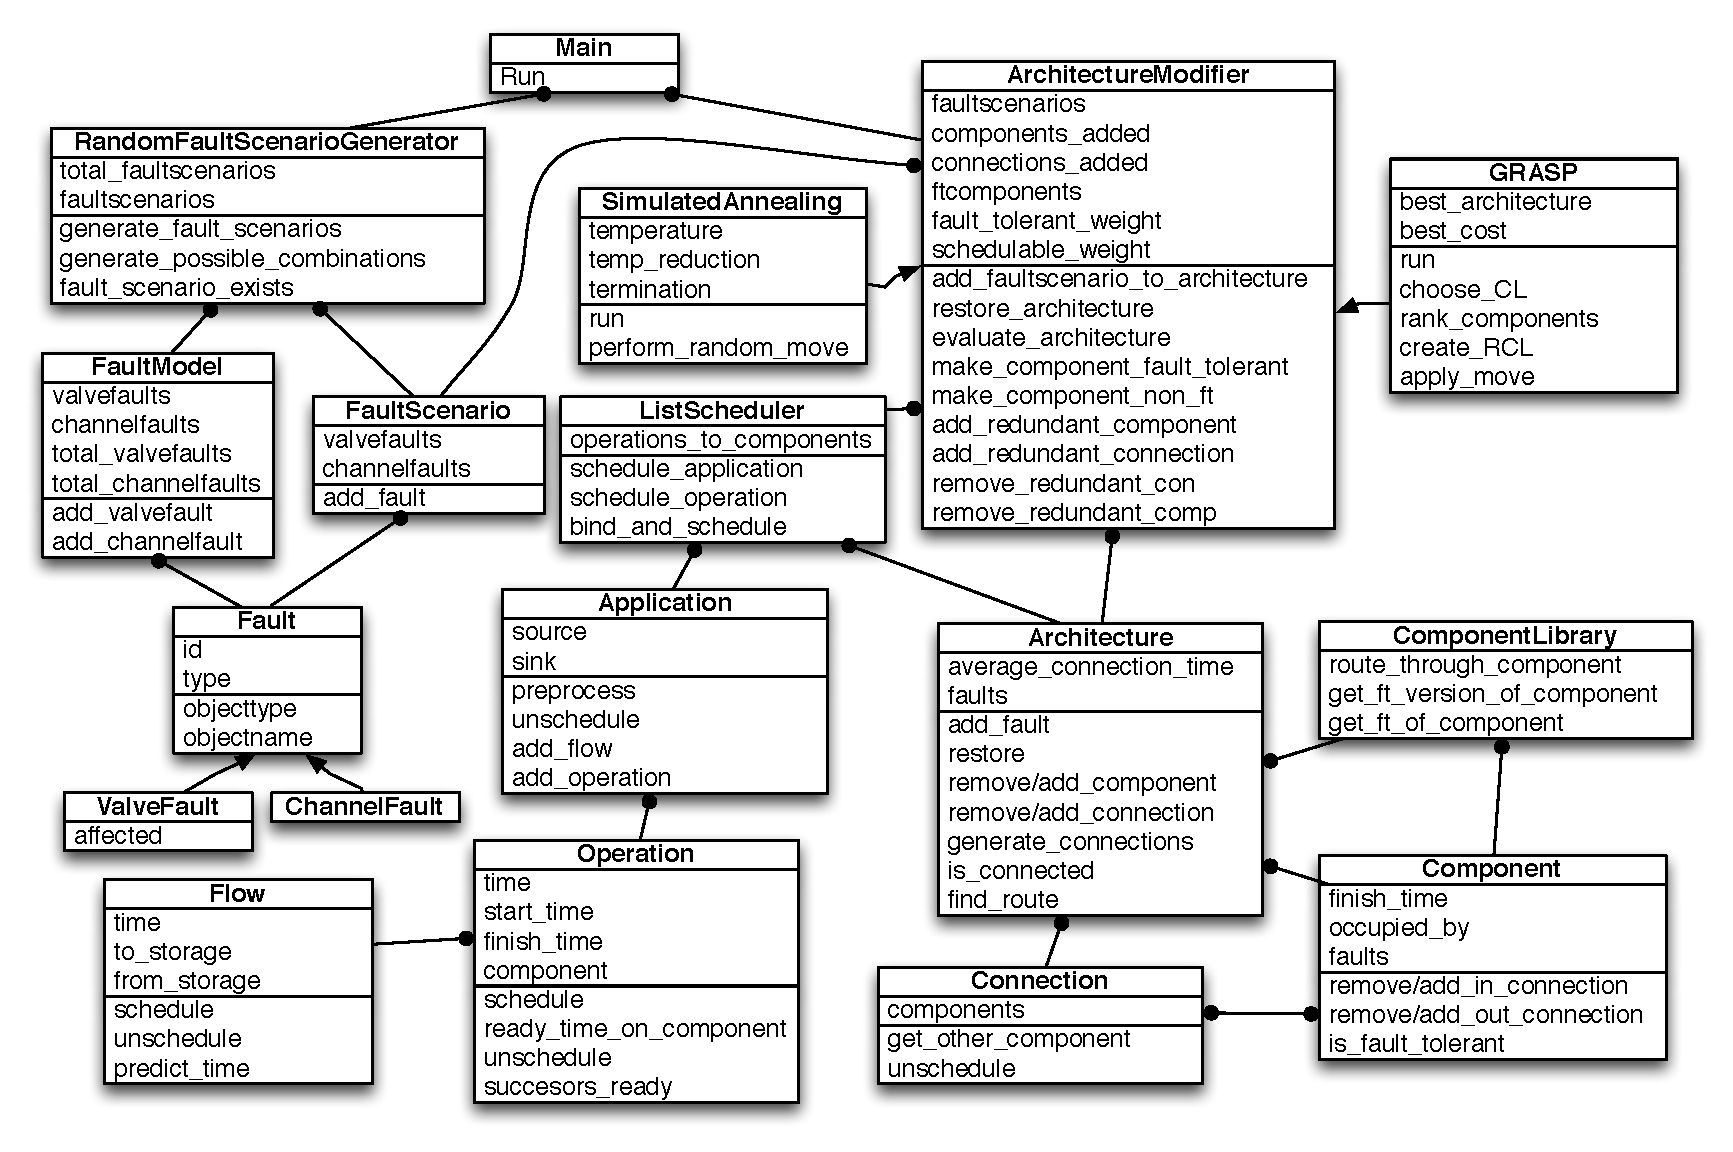
\includegraphics[scale=0.425]{figures/ClassDiagram.pdf}
\caption[Class diagram of the implementation]{Class diagram of the implementation}
\label{fig:class-diagram}
\end{figure}

In the following sections each module will be described and each class within the module will be clarified.

\subsection{Architecture}
The architecture module contains the classes for the architecture model, components, connections, component library and routes. The \emph{Architecture} class implements the architecture model and it has the responsibility of adding and removal of components and connections, finding routes for the fluid and generating the effects of faults. When finding routes between components, the architecture considers the effects of valve faults on switches, i.e. it might only be able to use certain connections if the valve is faulty. Similarly, the route search also considers blocked channels. Furthermore, it contains methods to add faults and restore from faults. The architecture uses the \emph{Component}, \emph{Connection} and \emph{ComponentLibrary} classes. The component class specify the type of the component, the in and out connections it has and furthermore it has scheduling related specifications. The connection class specify a simple graph edge and knows the two component it connects and it has details about scheduling. The reasoning behind components and connections having details about the scheduling is that it simplifies the scheduler, and unscheduling is also simple as it is just the resetting of used attributes. The component library has all the possible components and it keeps track of which components have and do not have fault-tolerance, the fault-tolerance of the components and which components they are the fault-tolerant version of.

\subsection{Fault Model}
The fault model module contains classes for the fault model, the faults, fault scenarios and the random generation of fault scenarios. The \emph{FaultModel} class is simple as it contains two sets which distinguish channel and valve faults, the maximum number of valve faults and the maximum number of channel faults. \emph{Fault} is a superclass which has two subclasses \emph{ValveFault} and \emph{ChannelFault}. The fault class specifies the object type the fault affects, either component or connection, and the name of component or connection, where the names of components and connections are specified in the JSON file for the architecture. The \emph{FaultScenario} class contains a set of valve faults and a set of channel faults. The \emph{RandomFaultScenarioGenerator} class implements the fault scenario generation algorithm described in detail in \autoref{sec:fs-gen}.

\subsection{Application}
The application module implements the application graph, the operations and the flows (edges) in the application graph. The \emph{Application} class contains a preprocess method for preprocessing the application graph and functionality to unschedule the application such it can be rescheduled and thereby a new schedule in the objective function can be found. The preprocessing consists of adding a source and a sink as operations to the graph. The source is added such that all the input operations depend on the source and the sink is added such that the sink depend on all the output operations. The \emph{Operation} class represent operations in the application graph. The class implements methods to find the ready time on specific components, which considers the routing time and constraints. The \emph{Flow} class model the dependencies (edges) in the application graph. The class implements methods to schedule the flows to storage and from storage if needed when scheduling, and they can easily be unscheduled.

\subsection{Parsing}
The parsing module contains all the parsers for the JSON files. The module contains a superclass named \emph{Parser}. In total, the tool receives 5 files and there is a class to parse each type of file, where all are subclasses of Parser. The \emph{ArchitectureParser} is responsible for parsing the netlist from the JSON file and create an object of the architecture class. Similarly, \emph{ApplicationParser}, \emph{ComponentLibraryParser}, \emph{FaultModelParser}, and \emph{ConfigParser} create the application graph, component library, fault model and the config data, respectively. The config data specifies the average routing latency, application deadline, number of fault scenarios, which algorithm to use and the algorithm specific details.

\subsection{Scheduling}
The scheduling module implements a superclass \emph{Scheduler} such that it is easily extendable to implement more schedulers if more schedulers are needed. The \emph{ListScheduler} class is a subclass of Scheduler. The ListScheduler class implements the List Scheduling algorithm which is described in detail in \autoref{sec:list-scheduling}.

\subsection{Architecture Modifier}
The architecture modifier module implements the design transformations, architecture evaluation, SA and GRASP. It has three classes \emph{ArchitectureModifier}, \emph{SimulatedAnnealing} and \emph{GRASP}. The ArchitectureModifier is a superclass which implements the design transformations, evaluates the architecture using the fault scenarios and keeps track of the added components, connections and fault-tolerant components converted. The moves are described in detail in \autoref{sec:moves}. Converting a component to fault-tolerant is simple as the type of the component just needs to be changed to the fault-tolerant type. Similar is the case, when converting it back to its regular version. When adding a connection, we just need to consider that the components do not get more incoming or outgoing channels than they are able to handle. Recall that a switch can only consist of four valves (channels) which also means that, e.g. a mixer cannot have more than two incoming and outgoing channels. Removing a connection is also simple as we keep track of the connections, we add to architecture and only redundant connections can be removed. Adding a redundant component however adds more complexity. The move is implemented such that the incoming and outgoing connections are always from / to switches. Consider the situation where all switches already have the maximum allowed channels, then two connections between two switches has to be modified to add a switch between them such that we can add the new component. Removing a redundant component therefore has to take this into consideration. It is implemented such that if a component has added switches to the architecture and we want to remove it, then it also removes the switches if, and only if, the switches do not have a connection to other components than the one, we wish to remove, and the switches from the connection, we modified. If the switches have connections to other components, they are kept in the architecture and added to the list of added components such that it is possible to remove. If it is removed later on, it will add the connection that we modified to the architecture.

Simulated Annealing and GRASP are subclasses of the ArchitectureModifier class as they use the moves and the architecture evaluation of their superclass. SA and GRASP are explained in detail in \autoref{sec:sa} and \autoref{sec:grasp}, respectively. The ArchitectureModifier superclass makes it easy to extend the tool with more algorithms to produce a fault-tolerant netlist that use the same moves and evaluation method.

\subsection{Serializing}
The serializing module contains two classes, a superclass \emph{Serializer} and a subclass \emph{NetlistSerializer}. This is to output the JSON file specifying the fault-tolerant netlist produced from this tool. The superclass is created such that it is easy to extend with more serializers, e.g. a serializer for applications. 

\subsection{Run}
The run module is the main file for running the program. It takes the command line input which is the JSON files specifying the initial netlist, application, fault model and config file.

\section{Testing}
The tool has been tested in an incremental manner as the different aspects was implemented. The scheduling was one of the first functionalities that was implemented. It was tested on different architectures with the associated application models using the architectures and applications provided by the work of \cite{wajid} and \cite{michael}. The example in \autoref{sec:prob-for} has been used as the key example for all steps in the implementation process. When the logic to generate faults was implemented, this example was used to test that the architecture responded in the correct way when finding routes and determining the connectivity of the architecture. Furthermore, we also tested how the faults affected the scheduling by affecting it both with faults that would make it impossible to schedule the application and contrary with faults where scheduling would still be possible. When it was determined that the effects of the faults were implemented correct, the moves were implemented. The moves were tested in different stages. First they were tested to see if when applied to an architecture the outcome was appropriate. When that test succeeded, it was then tested by affecting the architecture with faults that would affect connectivity and scheduling. Redundancy was then added to compensate for the faults and the outcome should be that the connectivity test and the scheduling would pass. After successfully implementing the moves, SA was implemented to use these moves and it was tested many times using the key example from \autoref{sec:prob-for} to make sure that the moves and their counter-moves were acting correctly when applied many times. GRASP was then implemented and tested similarly to SA.

\section{Summary}
This chapter outlines how the tool was implemented using a class diagram and explaining the different modules and classes. The implementation has been done such that it is easy to extend with new algorithms that will use the same objective function and moves as SA and GRASP and implement new scheduling algorithms. Similarly, every aspect of the tool is implemented. The testing was done incrementally where examples have been used to test every aspect of the tool. 
\chapter{Conclusions and Future Work}

\section{Conclusions}

\section{Future Work}
                                   %Chapter 1
%\chapter{Faults in Flow-Based Biochips}

\section{Possible Faults and Causes}

\section{Defects}

\section{Fault Modeling}

\section{Testing Strategy}

\section{Summary}                                 %Chapter 2
\appendix
\chapter{Stuff}

This appendix is full of stuff ...                                 %Appendix A
%-----------
% Backmatter
%-----------
\backmatter
\chaptermark{Bibliography}
\renewcommand{\sectionmark}[1]{\markright{#1}}
\sectionmark{Bibliography}
\addcontentsline{toc}{chapter}{Bibliography}        %Force addition of Bibliography to TOC
\bibliographystyle{alpha}                           %Use alpha codes for references
\bibliography{References}                           %Bibliography file called
\end{document}
% % % EOF % % %